{\Large Sound}
{
\definecolor{HumanAudioColor}{rgb}{0.2,0.2,0.6}
%
\begin{itemize}

\item Although sound, ocean waves, and heartbeats are not electromagnetic, they are included on this chart as a frequency reference. Other properties of electromagnetic waves are different from sound waves.

\item Sound waves are caused by an oscillating compression of molecules. Sound cannot travel in a vacuum such as outer space.

\item The speed of sound in air at sea level is 1240kph (770mph).

\item Humans can only hear sound between $\approx$20Hz to $\approx$20kHz.

\item Infrasound (below 20Hz) can be sensed by internal organs and touch.
%
%from http://www.worldtravelers.org/motionsickness.htm
Frequencies in the 0.2Hz range are often the cause of motion sickness.

\item Bats can hear sound up to $\approx$50kHz.

\item The 88 piano keys of the Equal Temperament scale are accurately located on the frequency chart.

\item Over the ages people have striven to divide the continuous audio frequency spectrum into individual musical notes that have harmonious relationships. Microtonal musicians study various scales. One recent count lists 4700 different musical scales.

\item The musical note A is depicted on the chart as \pscirclebox[fillstyle=solid,fillcolor=HumanAudioColor]{\textcolor{white}{A}}

\textcolor{gray}{\hrule}
\vspace{.1in}

%\item This image depicts air being compressed as sound waves in a tube from a speaker and then travelling through the tube towards the ear.\\
%%picture of sound
%\vspace{1.75in}
%\rput[t]{0}(1,-.5){%Description: Sound wave schematic travelling through air

\psset{unit=0.5in}

\psset{viewpoint=1 -1 1}

\definecolor{EarColour}{rgb}{1,0.8,0.8}

%Draw speaker
\ThreeDput[normal=1 0 0](0,0,0){
	\pscircle[fillstyle=solid,fillcolor=red,linecolor=red](0,0){0.4}
	}


\ThreeDput[normal=1 0 0](0.024,0,0){\pscircle[fillstyle=solid,fillcolor=green,linecolor=gray](0,0){0.3}}
\ThreeDput[normal=1 0 0](0.051,0,0){\pscircle[fillstyle=solid,fillcolor=green,linecolor=gray](0,0){0.3}}
\ThreeDput[normal=1 0 0](0.080,0,0){\pscircle[fillstyle=solid,fillcolor=green,linecolor=gray](0,0){0.3}}
\ThreeDput[normal=1 0 0](0.112,0,0){\pscircle[fillstyle=solid,fillcolor=green,linecolor=gray](0,0){0.3}}
\ThreeDput[normal=1 0 0](0.146,0,0){\pscircle[fillstyle=solid,fillcolor=green,linecolor=gray](0,0){0.3}}
\ThreeDput[normal=1 0 0](0.182,0,0){\pscircle[fillstyle=solid,fillcolor=green,linecolor=gray](0,0){0.3}}
\ThreeDput[normal=1 0 0](0.220,0,0){\pscircle[fillstyle=solid,fillcolor=green,linecolor=gray](0,0){0.3}}
\ThreeDput[normal=1 0 0](0.260,0,0){\pscircle[fillstyle=solid,fillcolor=green,linecolor=gray](0,0){0.3}}
\ThreeDput[normal=1 0 0](0.301,0,0){\pscircle[fillstyle=solid,fillcolor=green,linecolor=gray](0,0){0.3}}
\ThreeDput[normal=1 0 0](0.345,0,0){\pscircle[fillstyle=solid,fillcolor=green,linecolor=gray](0,0){0.3}}
\ThreeDput[normal=1 0 0](0.390,0,0){\pscircle[fillstyle=solid,fillcolor=green,linecolor=gray](0,0){0.3}}
\ThreeDput[normal=1 0 0](0.436,0,0){\pscircle[fillstyle=solid,fillcolor=green,linecolor=gray](0,0){0.3}}
\ThreeDput[normal=1 0 0](0.483,0,0){\pscircle[fillstyle=solid,fillcolor=green,linecolor=gray](0,0){0.3}}
\ThreeDput[normal=1 0 0](0.531,0,0){\pscircle[fillstyle=solid,fillcolor=green,linecolor=gray](0,0){0.3}}
\ThreeDput[normal=1 0 0](0.579,0,0){\pscircle[fillstyle=solid,fillcolor=green,linecolor=gray](0,0){0.3}}
\ThreeDput[normal=1 0 0](0.627,0,0){\pscircle[fillstyle=solid,fillcolor=green,linecolor=gray](0,0){0.3}}
\ThreeDput[normal=1 0 0](0.676,0,0){\pscircle[fillstyle=solid,fillcolor=green,linecolor=gray](0,0){0.3}}
\ThreeDput[normal=1 0 0](0.725,0,0){\pscircle[fillstyle=solid,fillcolor=green,linecolor=gray](0,0){0.3}}
\ThreeDput[normal=1 0 0](0.773,0,0){\pscircle[fillstyle=solid,fillcolor=green,linecolor=gray](0,0){0.3}}
\ThreeDput[normal=1 0 0](0.820,0,0){\pscircle[fillstyle=solid,fillcolor=green,linecolor=gray](0,0){0.3}}
\ThreeDput[normal=1 0 0](0.866,0,0){\pscircle[fillstyle=solid,fillcolor=green,linecolor=gray](0,0){0.3}}
\ThreeDput[normal=1 0 0](0.912,0,0){\pscircle[fillstyle=solid,fillcolor=green,linecolor=gray](0,0){0.3}}
\ThreeDput[normal=1 0 0](0.956,0,0){\pscircle[fillstyle=solid,fillcolor=green,linecolor=gray](0,0){0.3}}
\ThreeDput[normal=1 0 0](0.998,0,0){\pscircle[fillstyle=solid,fillcolor=green,linecolor=gray](0,0){0.3}}
\ThreeDput[normal=1 0 0](1.039,0,0){\pscircle[fillstyle=solid,fillcolor=green,linecolor=gray](0,0){0.3}}
\ThreeDput[normal=1 0 0](1.078,0,0){\pscircle[fillstyle=solid,fillcolor=green,linecolor=gray](0,0){0.3}}
\ThreeDput[normal=1 0 0](1.115,0,0){\pscircle[fillstyle=solid,fillcolor=green,linecolor=gray](0,0){0.3}}
\ThreeDput[normal=1 0 0](1.150,0,0){\pscircle[fillstyle=solid,fillcolor=green,linecolor=gray](0,0){0.3}}
\ThreeDput[normal=1 0 0](1.182,0,0){\pscircle[fillstyle=solid,fillcolor=green,linecolor=gray](0,0){0.3}}
\ThreeDput[normal=1 0 0](1.212,0,0){\pscircle[fillstyle=solid,fillcolor=green,linecolor=gray](0,0){0.3}}
\ThreeDput[normal=1 0 0](1.240,0,0){\pscircle[fillstyle=solid,fillcolor=green,linecolor=gray](0,0){0.3}}
\ThreeDput[normal=1 0 0](1.265,0,0){\pscircle[fillstyle=solid,fillcolor=green,linecolor=gray](0,0){0.3}}
\ThreeDput[normal=1 0 0](1.288,0,0){\pscircle[fillstyle=solid,fillcolor=green,linecolor=gray](0,0){0.3}}
\ThreeDput[normal=1 0 0](1.309,0,0){\pscircle[fillstyle=solid,fillcolor=green,linecolor=gray](0,0){0.3}}
\ThreeDput[normal=1 0 0](1.327,0,0){\pscircle[fillstyle=solid,fillcolor=green,linecolor=gray](0,0){0.3}}
\ThreeDput[normal=1 0 0](1.343,0,0){\pscircle[fillstyle=solid,fillcolor=green,linecolor=gray](0,0){0.3}}
\ThreeDput[normal=1 0 0](1.356,0,0){\pscircle[fillstyle=solid,fillcolor=green,linecolor=gray](0,0){0.3}}
\ThreeDput[normal=1 0 0](1.368,0,0){\pscircle[fillstyle=solid,fillcolor=green,linecolor=gray](0,0){0.3}}
\ThreeDput[normal=1 0 0](1.377,0,0){\pscircle[fillstyle=solid,fillcolor=green,linecolor=gray](0,0){0.3}}
\ThreeDput[normal=1 0 0](1.385,0,0){\pscircle[fillstyle=solid,fillcolor=green,linecolor=gray](0,0){0.3}}
\ThreeDput[normal=1 0 0](1.391,0,0){\pscircle[fillstyle=solid,fillcolor=green,linecolor=gray](0,0){0.3}}
\ThreeDput[normal=1 0 0](1.395,0,0){\pscircle[fillstyle=solid,fillcolor=green,linecolor=gray](0,0){0.3}}
\ThreeDput[normal=1 0 0](1.398,0,0){\pscircle[fillstyle=solid,fillcolor=green,linecolor=gray](0,0){0.3}}
\ThreeDput[normal=1 0 0](1.400,0,0){\pscircle[fillstyle=solid,fillcolor=green,linecolor=gray](0,0){0.3}}
\ThreeDput[normal=1 0 0](1.401,0,0){\pscircle[fillstyle=solid,fillcolor=green,linecolor=gray](0,0){0.3}}
\ThreeDput[normal=1 0 0](1.402,0,0){\pscircle[fillstyle=solid,fillcolor=green,linecolor=gray](0,0){0.3}}
\ThreeDput[normal=1 0 0](1.402,0,0){\pscircle[fillstyle=solid,fillcolor=green,linecolor=gray](0,0){0.3}}
\ThreeDput[normal=1 0 0](1.402,0,0){\pscircle[fillstyle=solid,fillcolor=green,linecolor=gray](0,0){0.3}}
\ThreeDput[normal=1 0 0](1.402,0,0){\pscircle[fillstyle=solid,fillcolor=green,linecolor=gray](0,0){0.3}}
\ThreeDput[normal=1 0 0](1.403,0,0){\pscircle[fillstyle=solid,fillcolor=green,linecolor=gray](0,0){0.3}}
\ThreeDput[normal=1 0 0](1.404,0,0){\pscircle[fillstyle=solid,fillcolor=green,linecolor=gray](0,0){0.3}}
\ThreeDput[normal=1 0 0](1.405,0,0){\pscircle[fillstyle=solid,fillcolor=green,linecolor=gray](0,0){0.3}}
\ThreeDput[normal=1 0 0](1.408,0,0){\pscircle[fillstyle=solid,fillcolor=green,linecolor=gray](0,0){0.3}}
\ThreeDput[normal=1 0 0](1.412,0,0){\pscircle[fillstyle=solid,fillcolor=green,linecolor=gray](0,0){0.3}}
\ThreeDput[normal=1 0 0](1.418,0,0){\pscircle[fillstyle=solid,fillcolor=green,linecolor=gray](0,0){0.3}}
\ThreeDput[normal=1 0 0](1.425,0,0){\pscircle[fillstyle=solid,fillcolor=green,linecolor=gray](0,0){0.3}}
\ThreeDput[normal=1 0 0](1.434,0,0){\pscircle[fillstyle=solid,fillcolor=green,linecolor=gray](0,0){0.3}}
\ThreeDput[normal=1 0 0](1.445,0,0){\pscircle[fillstyle=solid,fillcolor=green,linecolor=gray](0,0){0.3}}
\ThreeDput[normal=1 0 0](1.458,0,0){\pscircle[fillstyle=solid,fillcolor=green,linecolor=gray](0,0){0.3}}
\ThreeDput[normal=1 0 0](1.473,0,0){\pscircle[fillstyle=solid,fillcolor=green,linecolor=gray](0,0){0.3}}
\ThreeDput[normal=1 0 0](1.491,0,0){\pscircle[fillstyle=solid,fillcolor=green,linecolor=gray](0,0){0.3}}
\ThreeDput[normal=1 0 0](1.511,0,0){\pscircle[fillstyle=solid,fillcolor=green,linecolor=gray](0,0){0.3}}
\ThreeDput[normal=1 0 0](1.533,0,0){\pscircle[fillstyle=solid,fillcolor=green,linecolor=gray](0,0){0.3}}
\ThreeDput[normal=1 0 0](1.558,0,0){\pscircle[fillstyle=solid,fillcolor=green,linecolor=gray](0,0){0.3}}
\ThreeDput[normal=1 0 0](1.585,0,0){\pscircle[fillstyle=solid,fillcolor=green,linecolor=gray](0,0){0.3}}
\ThreeDput[normal=1 0 0](1.614,0,0){\pscircle[fillstyle=solid,fillcolor=green,linecolor=gray](0,0){0.3}}
\ThreeDput[normal=1 0 0](1.646,0,0){\pscircle[fillstyle=solid,fillcolor=green,linecolor=gray](0,0){0.3}}
\ThreeDput[normal=1 0 0](1.681,0,0){\pscircle[fillstyle=solid,fillcolor=green,linecolor=gray](0,0){0.3}}
\ThreeDput[normal=1 0 0](1.717,0,0){\pscircle[fillstyle=solid,fillcolor=green,linecolor=gray](0,0){0.3}}
\ThreeDput[normal=1 0 0](1.755,0,0){\pscircle[fillstyle=solid,fillcolor=green,linecolor=gray](0,0){0.3}}
\ThreeDput[normal=1 0 0](1.796,0,0){\pscircle[fillstyle=solid,fillcolor=green,linecolor=gray](0,0){0.3}}
\ThreeDput[normal=1 0 0](1.838,0,0){\pscircle[fillstyle=solid,fillcolor=green,linecolor=gray](0,0){0.3}}
\ThreeDput[normal=1 0 0](1.881,0,0){\pscircle[fillstyle=solid,fillcolor=green,linecolor=gray](0,0){0.3}}
\ThreeDput[normal=1 0 0](1.926,0,0){\pscircle[fillstyle=solid,fillcolor=green,linecolor=gray](0,0){0.3}}
\ThreeDput[normal=1 0 0](1.973,0,0){\pscircle[fillstyle=solid,fillcolor=green,linecolor=gray](0,0){0.3}}
\ThreeDput[normal=1 0 0](2.020,0,0){\pscircle[fillstyle=solid,fillcolor=green,linecolor=gray](0,0){0.3}}
\ThreeDput[normal=1 0 0](2.068,0,0){\pscircle[fillstyle=solid,fillcolor=green,linecolor=gray](0,0){0.3}}
\ThreeDput[normal=1 0 0](2.116,0,0){\pscircle[fillstyle=solid,fillcolor=green,linecolor=gray](0,0){0.3}}
\ThreeDput[normal=1 0 0](2.165,0,0){\pscircle[fillstyle=solid,fillcolor=green,linecolor=gray](0,0){0.3}}
\ThreeDput[normal=1 0 0](2.213,0,0){\pscircle[fillstyle=solid,fillcolor=green,linecolor=gray](0,0){0.3}}
\ThreeDput[normal=1 0 0](2.262,0,0){\pscircle[fillstyle=solid,fillcolor=green,linecolor=gray](0,0){0.3}}
\ThreeDput[normal=1 0 0](2.310,0,0){\pscircle[fillstyle=solid,fillcolor=green,linecolor=gray](0,0){0.3}}
\ThreeDput[normal=1 0 0](2.357,0,0){\pscircle[fillstyle=solid,fillcolor=green,linecolor=gray](0,0){0.3}}
\ThreeDput[normal=1 0 0](2.403,0,0){\pscircle[fillstyle=solid,fillcolor=green,linecolor=gray](0,0){0.3}}
\ThreeDput[normal=1 0 0](2.448,0,0){\pscircle[fillstyle=solid,fillcolor=green,linecolor=gray](0,0){0.3}}
\ThreeDput[normal=1 0 0](2.492,0,0){\pscircle[fillstyle=solid,fillcolor=green,linecolor=gray](0,0){0.3}}
\ThreeDput[normal=1 0 0](2.534,0,0){\pscircle[fillstyle=solid,fillcolor=green,linecolor=gray](0,0){0.3}}
\ThreeDput[normal=1 0 0](2.575,0,0){\pscircle[fillstyle=solid,fillcolor=green,linecolor=gray](0,0){0.3}}
\ThreeDput[normal=1 0 0](2.613,0,0){\pscircle[fillstyle=solid,fillcolor=green,linecolor=gray](0,0){0.3}}
\ThreeDput[normal=1 0 0](2.650,0,0){\pscircle[fillstyle=solid,fillcolor=green,linecolor=gray](0,0){0.3}}
\ThreeDput[normal=1 0 0](2.684,0,0){\pscircle[fillstyle=solid,fillcolor=green,linecolor=gray](0,0){0.3}}
\ThreeDput[normal=1 0 0](2.716,0,0){\pscircle[fillstyle=solid,fillcolor=green,linecolor=gray](0,0){0.3}}
\ThreeDput[normal=1 0 0](2.746,0,0){\pscircle[fillstyle=solid,fillcolor=green,linecolor=gray](0,0){0.3}}
\ThreeDput[normal=1 0 0](2.774,0,0){\pscircle[fillstyle=solid,fillcolor=green,linecolor=gray](0,0){0.3}}
\ThreeDput[normal=1 0 0](2.798,0,0){\pscircle[fillstyle=solid,fillcolor=green,linecolor=gray](0,0){0.3}}
\ThreeDput[normal=1 0 0](2.821,0,0){\pscircle[fillstyle=solid,fillcolor=green,linecolor=gray](0,0){0.3}}
\ThreeDput[normal=1 0 0](2.841,0,0){\pscircle[fillstyle=solid,fillcolor=green,linecolor=gray](0,0){0.3}}
\ThreeDput[normal=1 0 0](2.859,0,0){\pscircle[fillstyle=solid,fillcolor=green,linecolor=gray](0,0){0.3}}
\ThreeDput[normal=1 0 0](2.874,0,0){\pscircle[fillstyle=solid,fillcolor=green,linecolor=gray](0,0){0.3}}
\ThreeDput[normal=1 0 0](2.887,0,0){\pscircle[fillstyle=solid,fillcolor=green,linecolor=gray](0,0){0.3}}
\ThreeDput[normal=1 0 0](2.898,0,0){\pscircle[fillstyle=solid,fillcolor=green,linecolor=gray](0,0){0.3}}
\ThreeDput[normal=1 0 0](2.908,0,0){\pscircle[fillstyle=solid,fillcolor=green,linecolor=gray](0,0){0.3}}
\ThreeDput[normal=1 0 0](2.915,0,0){\pscircle[fillstyle=solid,fillcolor=green,linecolor=gray](0,0){0.3}}
\ThreeDput[normal=1 0 0](2.921,0,0){\pscircle[fillstyle=solid,fillcolor=green,linecolor=gray](0,0){0.3}}
\ThreeDput[normal=1 0 0](2.925,0,0){\pscircle[fillstyle=solid,fillcolor=green,linecolor=gray](0,0){0.3}}
\ThreeDput[normal=1 0 0](2.928,0,0){\pscircle[fillstyle=solid,fillcolor=green,linecolor=gray](0,0){0.3}}
\ThreeDput[normal=1 0 0](2.930,0,0){\pscircle[fillstyle=solid,fillcolor=green,linecolor=gray](0,0){0.3}}
\ThreeDput[normal=1 0 0](2.931,0,0){\pscircle[fillstyle=solid,fillcolor=green,linecolor=gray](0,0){0.3}}
\ThreeDput[normal=1 0 0](2.931,0,0){\pscircle[fillstyle=solid,fillcolor=green,linecolor=gray](0,0){0.3}}
\ThreeDput[normal=1 0 0](2.931,0,0){\pscircle[fillstyle=solid,fillcolor=green,linecolor=gray](0,0){0.3}}
\ThreeDput[normal=1 0 0](2.931,0,0){\pscircle[fillstyle=solid,fillcolor=green,linecolor=gray](0,0){0.3}}
\ThreeDput[normal=1 0 0](2.931,0,0){\pscircle[fillstyle=solid,fillcolor=green,linecolor=gray](0,0){0.3}}
\ThreeDput[normal=1 0 0](2.932,0,0){\pscircle[fillstyle=solid,fillcolor=green,linecolor=gray](0,0){0.3}}
\ThreeDput[normal=1 0 0](2.933,0,0){\pscircle[fillstyle=solid,fillcolor=green,linecolor=gray](0,0){0.3}}
\ThreeDput[normal=1 0 0](2.935,0,0){\pscircle[fillstyle=solid,fillcolor=green,linecolor=gray](0,0){0.3}}
\ThreeDput[normal=1 0 0](2.938,0,0){\pscircle[fillstyle=solid,fillcolor=green,linecolor=gray](0,0){0.3}}
\ThreeDput[normal=1 0 0](2.942,0,0){\pscircle[fillstyle=solid,fillcolor=green,linecolor=gray](0,0){0.3}}
\ThreeDput[normal=1 0 0](2.948,0,0){\pscircle[fillstyle=solid,fillcolor=green,linecolor=gray](0,0){0.3}}
\ThreeDput[normal=1 0 0](2.956,0,0){\pscircle[fillstyle=solid,fillcolor=green,linecolor=gray](0,0){0.3}}
\ThreeDput[normal=1 0 0](2.965,0,0){\pscircle[fillstyle=solid,fillcolor=green,linecolor=gray](0,0){0.3}}
\ThreeDput[normal=1 0 0](2.976,0,0){\pscircle[fillstyle=solid,fillcolor=green,linecolor=gray](0,0){0.3}}
\ThreeDput[normal=1 0 0](2.989,0,0){\pscircle[fillstyle=solid,fillcolor=green,linecolor=gray](0,0){0.3}}
\ThreeDput[normal=1 0 0](3.005,0,0){\pscircle[fillstyle=solid,fillcolor=green,linecolor=gray](0,0){0.3}}
\ThreeDput[normal=1 0 0](3.023,0,0){\pscircle[fillstyle=solid,fillcolor=green,linecolor=gray](0,0){0.3}}
\ThreeDput[normal=1 0 0](3.043,0,0){\pscircle[fillstyle=solid,fillcolor=green,linecolor=gray](0,0){0.3}}
\ThreeDput[normal=1 0 0](3.066,0,0){\pscircle[fillstyle=solid,fillcolor=green,linecolor=gray](0,0){0.3}}
\ThreeDput[normal=1 0 0](3.091,0,0){\pscircle[fillstyle=solid,fillcolor=green,linecolor=gray](0,0){0.3}}
\ThreeDput[normal=1 0 0](3.119,0,0){\pscircle[fillstyle=solid,fillcolor=green,linecolor=gray](0,0){0.3}}
\ThreeDput[normal=1 0 0](3.149,0,0){\pscircle[fillstyle=solid,fillcolor=green,linecolor=gray](0,0){0.3}}
\ThreeDput[normal=1 0 0](3.181,0,0){\pscircle[fillstyle=solid,fillcolor=green,linecolor=gray](0,0){0.3}}
\ThreeDput[normal=1 0 0](3.216,0,0){\pscircle[fillstyle=solid,fillcolor=green,linecolor=gray](0,0){0.3}}
\ThreeDput[normal=1 0 0](3.252,0,0){\pscircle[fillstyle=solid,fillcolor=green,linecolor=gray](0,0){0.3}}
\ThreeDput[normal=1 0 0](3.291,0,0){\pscircle[fillstyle=solid,fillcolor=green,linecolor=gray](0,0){0.3}}
\ThreeDput[normal=1 0 0](3.332,0,0){\pscircle[fillstyle=solid,fillcolor=green,linecolor=gray](0,0){0.3}}
\ThreeDput[normal=1 0 0](3.374,0,0){\pscircle[fillstyle=solid,fillcolor=green,linecolor=gray](0,0){0.3}}
\ThreeDput[normal=1 0 0](3.418,0,0){\pscircle[fillstyle=solid,fillcolor=green,linecolor=gray](0,0){0.3}}
\ThreeDput[normal=1 0 0](3.463,0,0){\pscircle[fillstyle=solid,fillcolor=green,linecolor=gray](0,0){0.3}}
\ThreeDput[normal=1 0 0](3.510,0,0){\pscircle[fillstyle=solid,fillcolor=green,linecolor=gray](0,0){0.3}}
\ThreeDput[normal=1 0 0](3.557,0,0){\pscircle[fillstyle=solid,fillcolor=green,linecolor=gray](0,0){0.3}}
\ThreeDput[normal=1 0 0](3.605,0,0){\pscircle[fillstyle=solid,fillcolor=green,linecolor=gray](0,0){0.3}}
\ThreeDput[normal=1 0 0](3.653,0,0){\pscircle[fillstyle=solid,fillcolor=green,linecolor=gray](0,0){0.3}}
\ThreeDput[normal=1 0 0](3.702,0,0){\pscircle[fillstyle=solid,fillcolor=green,linecolor=gray](0,0){0.3}}
\ThreeDput[normal=1 0 0](3.751,0,0){\pscircle[fillstyle=solid,fillcolor=green,linecolor=gray](0,0){0.3}}
\ThreeDput[normal=1 0 0](3.799,0,0){\pscircle[fillstyle=solid,fillcolor=green,linecolor=gray](0,0){0.3}}
\ThreeDput[normal=1 0 0](3.847,0,0){\pscircle[fillstyle=solid,fillcolor=green,linecolor=gray](0,0){0.3}}
\ThreeDput[normal=1 0 0](3.894,0,0){\pscircle[fillstyle=solid,fillcolor=green,linecolor=gray](0,0){0.3}}
\ThreeDput[normal=1 0 0](3.940,0,0){\pscircle[fillstyle=solid,fillcolor=green,linecolor=gray](0,0){0.3}}
\ThreeDput[normal=1 0 0](3.985,0,0){\pscircle[fillstyle=solid,fillcolor=green,linecolor=gray](0,0){0.3}}
\ThreeDput[normal=1 0 0](4.028,0,0){\pscircle[fillstyle=solid,fillcolor=green,linecolor=gray](0,0){0.3}}
\ThreeDput[normal=1 0 0](4.070,0,0){\pscircle[fillstyle=solid,fillcolor=green,linecolor=gray](0,0){0.3}}
\ThreeDput[normal=1 0 0](4.111,0,0){\pscircle[fillstyle=solid,fillcolor=green,linecolor=gray](0,0){0.3}}
\ThreeDput[normal=1 0 0](4.149,0,0){\pscircle[fillstyle=solid,fillcolor=green,linecolor=gray](0,0){0.3}}
\ThreeDput[normal=1 0 0](4.185,0,0){\pscircle[fillstyle=solid,fillcolor=green,linecolor=gray](0,0){0.3}}
\ThreeDput[normal=1 0 0](4.219,0,0){\pscircle[fillstyle=solid,fillcolor=green,linecolor=gray](0,0){0.3}}
\ThreeDput[normal=1 0 0](4.251,0,0){\pscircle[fillstyle=solid,fillcolor=green,linecolor=gray](0,0){0.3}}
\ThreeDput[normal=1 0 0](4.280,0,0){\pscircle[fillstyle=solid,fillcolor=green,linecolor=gray](0,0){0.3}}
\ThreeDput[normal=1 0 0](4.307,0,0){\pscircle[fillstyle=solid,fillcolor=green,linecolor=gray](0,0){0.3}}
\ThreeDput[normal=1 0 0](4.331,0,0){\pscircle[fillstyle=solid,fillcolor=green,linecolor=gray](0,0){0.3}}
\ThreeDput[normal=1 0 0](4.354,0,0){\pscircle[fillstyle=solid,fillcolor=green,linecolor=gray](0,0){0.3}}
\ThreeDput[normal=1 0 0](4.373,0,0){\pscircle[fillstyle=solid,fillcolor=green,linecolor=gray](0,0){0.3}}
\ThreeDput[normal=1 0 0](4.391,0,0){\pscircle[fillstyle=solid,fillcolor=green,linecolor=gray](0,0){0.3}}
\ThreeDput[normal=1 0 0](4.406,0,0){\pscircle[fillstyle=solid,fillcolor=green,linecolor=gray](0,0){0.3}}
\ThreeDput[normal=1 0 0](4.418,0,0){\pscircle[fillstyle=solid,fillcolor=green,linecolor=gray](0,0){0.3}}
\ThreeDput[normal=1 0 0](4.429,0,0){\pscircle[fillstyle=solid,fillcolor=green,linecolor=gray](0,0){0.3}}
\ThreeDput[normal=1 0 0](4.438,0,0){\pscircle[fillstyle=solid,fillcolor=green,linecolor=gray](0,0){0.3}}
\ThreeDput[normal=1 0 0](4.445,0,0){\pscircle[fillstyle=solid,fillcolor=green,linecolor=gray](0,0){0.3}}
\ThreeDput[normal=1 0 0](4.450,0,0){\pscircle[fillstyle=solid,fillcolor=green,linecolor=gray](0,0){0.3}}
\ThreeDput[normal=1 0 0](4.454,0,0){\pscircle[fillstyle=solid,fillcolor=green,linecolor=gray](0,0){0.3}}
\ThreeDput[normal=1 0 0](4.457,0,0){\pscircle[fillstyle=solid,fillcolor=green,linecolor=gray](0,0){0.3}}
\ThreeDput[normal=1 0 0](4.459,0,0){\pscircle[fillstyle=solid,fillcolor=green,linecolor=gray](0,0){0.3}}
\ThreeDput[normal=1 0 0](4.460,0,0){\pscircle[fillstyle=solid,fillcolor=green,linecolor=gray](0,0){0.3}}
\ThreeDput[normal=1 0 0](4.460,0,0){\pscircle[fillstyle=solid,fillcolor=green,linecolor=gray](0,0){0.3}}
\ThreeDput[normal=1 0 0](4.460,0,0){\pscircle[fillstyle=solid,fillcolor=green,linecolor=gray](0,0){0.3}}
\ThreeDput[normal=1 0 0](4.460,0,0){\pscircle[fillstyle=solid,fillcolor=green,linecolor=gray](0,0){0.3}}
\ThreeDput[normal=1 0 0](4.460,0,0){\pscircle[fillstyle=solid,fillcolor=green,linecolor=gray](0,0){0.3}}
\ThreeDput[normal=1 0 0](4.461,0,0){\pscircle[fillstyle=solid,fillcolor=green,linecolor=gray](0,0){0.3}}
\ThreeDput[normal=1 0 0](4.462,0,0){\pscircle[fillstyle=solid,fillcolor=green,linecolor=gray](0,0){0.3}}
\ThreeDput[normal=1 0 0](4.464,0,0){\pscircle[fillstyle=solid,fillcolor=green,linecolor=gray](0,0){0.3}}
\ThreeDput[normal=1 0 0](4.468,0,0){\pscircle[fillstyle=solid,fillcolor=green,linecolor=gray](0,0){0.3}}
\ThreeDput[normal=1 0 0](4.472,0,0){\pscircle[fillstyle=solid,fillcolor=green,linecolor=gray](0,0){0.3}}
\ThreeDput[normal=1 0 0](4.478,0,0){\pscircle[fillstyle=solid,fillcolor=green,linecolor=gray](0,0){0.3}}
\ThreeDput[normal=1 0 0](4.486,0,0){\pscircle[fillstyle=solid,fillcolor=green,linecolor=gray](0,0){0.3}}
\ThreeDput[normal=1 0 0](4.496,0,0){\pscircle[fillstyle=solid,fillcolor=green,linecolor=gray](0,0){0.3}}
\ThreeDput[normal=1 0 0](4.507,0,0){\pscircle[fillstyle=solid,fillcolor=green,linecolor=gray](0,0){0.3}}
\ThreeDput[normal=1 0 0](4.521,0,0){\pscircle[fillstyle=solid,fillcolor=green,linecolor=gray](0,0){0.3}}
\ThreeDput[normal=1 0 0](4.537,0,0){\pscircle[fillstyle=solid,fillcolor=green,linecolor=gray](0,0){0.3}}
\ThreeDput[normal=1 0 0](4.555,0,0){\pscircle[fillstyle=solid,fillcolor=green,linecolor=gray](0,0){0.3}}
\ThreeDput[normal=1 0 0](4.576,0,0){\pscircle[fillstyle=solid,fillcolor=green,linecolor=gray](0,0){0.3}}
\ThreeDput[normal=1 0 0](4.599,0,0){\pscircle[fillstyle=solid,fillcolor=green,linecolor=gray](0,0){0.3}}
\ThreeDput[normal=1 0 0](4.625,0,0){\pscircle[fillstyle=solid,fillcolor=green,linecolor=gray](0,0){0.3}}
\ThreeDput[normal=1 0 0](4.653,0,0){\pscircle[fillstyle=solid,fillcolor=green,linecolor=gray](0,0){0.3}}
\ThreeDput[normal=1 0 0](4.683,0,0){\pscircle[fillstyle=solid,fillcolor=green,linecolor=gray](0,0){0.3}}
\ThreeDput[normal=1 0 0](4.716,0,0){\pscircle[fillstyle=solid,fillcolor=green,linecolor=gray](0,0){0.3}}
\ThreeDput[normal=1 0 0](4.751,0,0){\pscircle[fillstyle=solid,fillcolor=green,linecolor=gray](0,0){0.3}}
\ThreeDput[normal=1 0 0](4.788,0,0){\pscircle[fillstyle=solid,fillcolor=green,linecolor=gray](0,0){0.3}}
\ThreeDput[normal=1 0 0](4.827,0,0){\pscircle[fillstyle=solid,fillcolor=green,linecolor=gray](0,0){0.3}}
\ThreeDput[normal=1 0 0](4.868,0,0){\pscircle[fillstyle=solid,fillcolor=green,linecolor=gray](0,0){0.3}}
\ThreeDput[normal=1 0 0](4.910,0,0){\pscircle[fillstyle=solid,fillcolor=green,linecolor=gray](0,0){0.3}}
\ThreeDput[normal=1 0 0](4.955,0,0){\pscircle[fillstyle=solid,fillcolor=green,linecolor=gray](0,0){0.3}}
\ThreeDput[normal=1 0 0](5.000,0,0){\pscircle[fillstyle=solid,fillcolor=green,linecolor=gray](0,0){0.3}}


% Speaker label
\ThreeDput[normal=0 -1 0]{
	\uput{0.2in}[180](0,0){\white Speaker}
	}

%Draw ear
\ThreeDput[normal=1 0 0](5,0,0){
	\pscircle[fillstyle=solid,fillcolor=EarColour,linecolor=gray](0,0){0.4}
	}



% Ear label
\ThreeDput[normal=1 0 0](5,0,0){
	\rput(0,0){Ear}
	}
}
\end{itemize}
	\vspace{0.1in}
	%
	\begin{tabular}{rl}
	%\begin{minipage}[b]{2.45in}\rput(.65,1){%Description: Sound wave schematic travelling through air

\psset{unit=0.5in}

\psset{viewpoint=1 -1 1}

\definecolor{EarColour}{rgb}{1,0.8,0.8}

%Draw speaker
\ThreeDput[normal=1 0 0](0,0,0){
	\pscircle[fillstyle=solid,fillcolor=red,linecolor=red](0,0){0.4}
	}


\ThreeDput[normal=1 0 0](0.024,0,0){\pscircle[fillstyle=solid,fillcolor=green,linecolor=gray](0,0){0.3}}
\ThreeDput[normal=1 0 0](0.051,0,0){\pscircle[fillstyle=solid,fillcolor=green,linecolor=gray](0,0){0.3}}
\ThreeDput[normal=1 0 0](0.080,0,0){\pscircle[fillstyle=solid,fillcolor=green,linecolor=gray](0,0){0.3}}
\ThreeDput[normal=1 0 0](0.112,0,0){\pscircle[fillstyle=solid,fillcolor=green,linecolor=gray](0,0){0.3}}
\ThreeDput[normal=1 0 0](0.146,0,0){\pscircle[fillstyle=solid,fillcolor=green,linecolor=gray](0,0){0.3}}
\ThreeDput[normal=1 0 0](0.182,0,0){\pscircle[fillstyle=solid,fillcolor=green,linecolor=gray](0,0){0.3}}
\ThreeDput[normal=1 0 0](0.220,0,0){\pscircle[fillstyle=solid,fillcolor=green,linecolor=gray](0,0){0.3}}
\ThreeDput[normal=1 0 0](0.260,0,0){\pscircle[fillstyle=solid,fillcolor=green,linecolor=gray](0,0){0.3}}
\ThreeDput[normal=1 0 0](0.301,0,0){\pscircle[fillstyle=solid,fillcolor=green,linecolor=gray](0,0){0.3}}
\ThreeDput[normal=1 0 0](0.345,0,0){\pscircle[fillstyle=solid,fillcolor=green,linecolor=gray](0,0){0.3}}
\ThreeDput[normal=1 0 0](0.390,0,0){\pscircle[fillstyle=solid,fillcolor=green,linecolor=gray](0,0){0.3}}
\ThreeDput[normal=1 0 0](0.436,0,0){\pscircle[fillstyle=solid,fillcolor=green,linecolor=gray](0,0){0.3}}
\ThreeDput[normal=1 0 0](0.483,0,0){\pscircle[fillstyle=solid,fillcolor=green,linecolor=gray](0,0){0.3}}
\ThreeDput[normal=1 0 0](0.531,0,0){\pscircle[fillstyle=solid,fillcolor=green,linecolor=gray](0,0){0.3}}
\ThreeDput[normal=1 0 0](0.579,0,0){\pscircle[fillstyle=solid,fillcolor=green,linecolor=gray](0,0){0.3}}
\ThreeDput[normal=1 0 0](0.627,0,0){\pscircle[fillstyle=solid,fillcolor=green,linecolor=gray](0,0){0.3}}
\ThreeDput[normal=1 0 0](0.676,0,0){\pscircle[fillstyle=solid,fillcolor=green,linecolor=gray](0,0){0.3}}
\ThreeDput[normal=1 0 0](0.725,0,0){\pscircle[fillstyle=solid,fillcolor=green,linecolor=gray](0,0){0.3}}
\ThreeDput[normal=1 0 0](0.773,0,0){\pscircle[fillstyle=solid,fillcolor=green,linecolor=gray](0,0){0.3}}
\ThreeDput[normal=1 0 0](0.820,0,0){\pscircle[fillstyle=solid,fillcolor=green,linecolor=gray](0,0){0.3}}
\ThreeDput[normal=1 0 0](0.866,0,0){\pscircle[fillstyle=solid,fillcolor=green,linecolor=gray](0,0){0.3}}
\ThreeDput[normal=1 0 0](0.912,0,0){\pscircle[fillstyle=solid,fillcolor=green,linecolor=gray](0,0){0.3}}
\ThreeDput[normal=1 0 0](0.956,0,0){\pscircle[fillstyle=solid,fillcolor=green,linecolor=gray](0,0){0.3}}
\ThreeDput[normal=1 0 0](0.998,0,0){\pscircle[fillstyle=solid,fillcolor=green,linecolor=gray](0,0){0.3}}
\ThreeDput[normal=1 0 0](1.039,0,0){\pscircle[fillstyle=solid,fillcolor=green,linecolor=gray](0,0){0.3}}
\ThreeDput[normal=1 0 0](1.078,0,0){\pscircle[fillstyle=solid,fillcolor=green,linecolor=gray](0,0){0.3}}
\ThreeDput[normal=1 0 0](1.115,0,0){\pscircle[fillstyle=solid,fillcolor=green,linecolor=gray](0,0){0.3}}
\ThreeDput[normal=1 0 0](1.150,0,0){\pscircle[fillstyle=solid,fillcolor=green,linecolor=gray](0,0){0.3}}
\ThreeDput[normal=1 0 0](1.182,0,0){\pscircle[fillstyle=solid,fillcolor=green,linecolor=gray](0,0){0.3}}
\ThreeDput[normal=1 0 0](1.212,0,0){\pscircle[fillstyle=solid,fillcolor=green,linecolor=gray](0,0){0.3}}
\ThreeDput[normal=1 0 0](1.240,0,0){\pscircle[fillstyle=solid,fillcolor=green,linecolor=gray](0,0){0.3}}
\ThreeDput[normal=1 0 0](1.265,0,0){\pscircle[fillstyle=solid,fillcolor=green,linecolor=gray](0,0){0.3}}
\ThreeDput[normal=1 0 0](1.288,0,0){\pscircle[fillstyle=solid,fillcolor=green,linecolor=gray](0,0){0.3}}
\ThreeDput[normal=1 0 0](1.309,0,0){\pscircle[fillstyle=solid,fillcolor=green,linecolor=gray](0,0){0.3}}
\ThreeDput[normal=1 0 0](1.327,0,0){\pscircle[fillstyle=solid,fillcolor=green,linecolor=gray](0,0){0.3}}
\ThreeDput[normal=1 0 0](1.343,0,0){\pscircle[fillstyle=solid,fillcolor=green,linecolor=gray](0,0){0.3}}
\ThreeDput[normal=1 0 0](1.356,0,0){\pscircle[fillstyle=solid,fillcolor=green,linecolor=gray](0,0){0.3}}
\ThreeDput[normal=1 0 0](1.368,0,0){\pscircle[fillstyle=solid,fillcolor=green,linecolor=gray](0,0){0.3}}
\ThreeDput[normal=1 0 0](1.377,0,0){\pscircle[fillstyle=solid,fillcolor=green,linecolor=gray](0,0){0.3}}
\ThreeDput[normal=1 0 0](1.385,0,0){\pscircle[fillstyle=solid,fillcolor=green,linecolor=gray](0,0){0.3}}
\ThreeDput[normal=1 0 0](1.391,0,0){\pscircle[fillstyle=solid,fillcolor=green,linecolor=gray](0,0){0.3}}
\ThreeDput[normal=1 0 0](1.395,0,0){\pscircle[fillstyle=solid,fillcolor=green,linecolor=gray](0,0){0.3}}
\ThreeDput[normal=1 0 0](1.398,0,0){\pscircle[fillstyle=solid,fillcolor=green,linecolor=gray](0,0){0.3}}
\ThreeDput[normal=1 0 0](1.400,0,0){\pscircle[fillstyle=solid,fillcolor=green,linecolor=gray](0,0){0.3}}
\ThreeDput[normal=1 0 0](1.401,0,0){\pscircle[fillstyle=solid,fillcolor=green,linecolor=gray](0,0){0.3}}
\ThreeDput[normal=1 0 0](1.402,0,0){\pscircle[fillstyle=solid,fillcolor=green,linecolor=gray](0,0){0.3}}
\ThreeDput[normal=1 0 0](1.402,0,0){\pscircle[fillstyle=solid,fillcolor=green,linecolor=gray](0,0){0.3}}
\ThreeDput[normal=1 0 0](1.402,0,0){\pscircle[fillstyle=solid,fillcolor=green,linecolor=gray](0,0){0.3}}
\ThreeDput[normal=1 0 0](1.402,0,0){\pscircle[fillstyle=solid,fillcolor=green,linecolor=gray](0,0){0.3}}
\ThreeDput[normal=1 0 0](1.403,0,0){\pscircle[fillstyle=solid,fillcolor=green,linecolor=gray](0,0){0.3}}
\ThreeDput[normal=1 0 0](1.404,0,0){\pscircle[fillstyle=solid,fillcolor=green,linecolor=gray](0,0){0.3}}
\ThreeDput[normal=1 0 0](1.405,0,0){\pscircle[fillstyle=solid,fillcolor=green,linecolor=gray](0,0){0.3}}
\ThreeDput[normal=1 0 0](1.408,0,0){\pscircle[fillstyle=solid,fillcolor=green,linecolor=gray](0,0){0.3}}
\ThreeDput[normal=1 0 0](1.412,0,0){\pscircle[fillstyle=solid,fillcolor=green,linecolor=gray](0,0){0.3}}
\ThreeDput[normal=1 0 0](1.418,0,0){\pscircle[fillstyle=solid,fillcolor=green,linecolor=gray](0,0){0.3}}
\ThreeDput[normal=1 0 0](1.425,0,0){\pscircle[fillstyle=solid,fillcolor=green,linecolor=gray](0,0){0.3}}
\ThreeDput[normal=1 0 0](1.434,0,0){\pscircle[fillstyle=solid,fillcolor=green,linecolor=gray](0,0){0.3}}
\ThreeDput[normal=1 0 0](1.445,0,0){\pscircle[fillstyle=solid,fillcolor=green,linecolor=gray](0,0){0.3}}
\ThreeDput[normal=1 0 0](1.458,0,0){\pscircle[fillstyle=solid,fillcolor=green,linecolor=gray](0,0){0.3}}
\ThreeDput[normal=1 0 0](1.473,0,0){\pscircle[fillstyle=solid,fillcolor=green,linecolor=gray](0,0){0.3}}
\ThreeDput[normal=1 0 0](1.491,0,0){\pscircle[fillstyle=solid,fillcolor=green,linecolor=gray](0,0){0.3}}
\ThreeDput[normal=1 0 0](1.511,0,0){\pscircle[fillstyle=solid,fillcolor=green,linecolor=gray](0,0){0.3}}
\ThreeDput[normal=1 0 0](1.533,0,0){\pscircle[fillstyle=solid,fillcolor=green,linecolor=gray](0,0){0.3}}
\ThreeDput[normal=1 0 0](1.558,0,0){\pscircle[fillstyle=solid,fillcolor=green,linecolor=gray](0,0){0.3}}
\ThreeDput[normal=1 0 0](1.585,0,0){\pscircle[fillstyle=solid,fillcolor=green,linecolor=gray](0,0){0.3}}
\ThreeDput[normal=1 0 0](1.614,0,0){\pscircle[fillstyle=solid,fillcolor=green,linecolor=gray](0,0){0.3}}
\ThreeDput[normal=1 0 0](1.646,0,0){\pscircle[fillstyle=solid,fillcolor=green,linecolor=gray](0,0){0.3}}
\ThreeDput[normal=1 0 0](1.681,0,0){\pscircle[fillstyle=solid,fillcolor=green,linecolor=gray](0,0){0.3}}
\ThreeDput[normal=1 0 0](1.717,0,0){\pscircle[fillstyle=solid,fillcolor=green,linecolor=gray](0,0){0.3}}
\ThreeDput[normal=1 0 0](1.755,0,0){\pscircle[fillstyle=solid,fillcolor=green,linecolor=gray](0,0){0.3}}
\ThreeDput[normal=1 0 0](1.796,0,0){\pscircle[fillstyle=solid,fillcolor=green,linecolor=gray](0,0){0.3}}
\ThreeDput[normal=1 0 0](1.838,0,0){\pscircle[fillstyle=solid,fillcolor=green,linecolor=gray](0,0){0.3}}
\ThreeDput[normal=1 0 0](1.881,0,0){\pscircle[fillstyle=solid,fillcolor=green,linecolor=gray](0,0){0.3}}
\ThreeDput[normal=1 0 0](1.926,0,0){\pscircle[fillstyle=solid,fillcolor=green,linecolor=gray](0,0){0.3}}
\ThreeDput[normal=1 0 0](1.973,0,0){\pscircle[fillstyle=solid,fillcolor=green,linecolor=gray](0,0){0.3}}
\ThreeDput[normal=1 0 0](2.020,0,0){\pscircle[fillstyle=solid,fillcolor=green,linecolor=gray](0,0){0.3}}
\ThreeDput[normal=1 0 0](2.068,0,0){\pscircle[fillstyle=solid,fillcolor=green,linecolor=gray](0,0){0.3}}
\ThreeDput[normal=1 0 0](2.116,0,0){\pscircle[fillstyle=solid,fillcolor=green,linecolor=gray](0,0){0.3}}
\ThreeDput[normal=1 0 0](2.165,0,0){\pscircle[fillstyle=solid,fillcolor=green,linecolor=gray](0,0){0.3}}
\ThreeDput[normal=1 0 0](2.213,0,0){\pscircle[fillstyle=solid,fillcolor=green,linecolor=gray](0,0){0.3}}
\ThreeDput[normal=1 0 0](2.262,0,0){\pscircle[fillstyle=solid,fillcolor=green,linecolor=gray](0,0){0.3}}
\ThreeDput[normal=1 0 0](2.310,0,0){\pscircle[fillstyle=solid,fillcolor=green,linecolor=gray](0,0){0.3}}
\ThreeDput[normal=1 0 0](2.357,0,0){\pscircle[fillstyle=solid,fillcolor=green,linecolor=gray](0,0){0.3}}
\ThreeDput[normal=1 0 0](2.403,0,0){\pscircle[fillstyle=solid,fillcolor=green,linecolor=gray](0,0){0.3}}
\ThreeDput[normal=1 0 0](2.448,0,0){\pscircle[fillstyle=solid,fillcolor=green,linecolor=gray](0,0){0.3}}
\ThreeDput[normal=1 0 0](2.492,0,0){\pscircle[fillstyle=solid,fillcolor=green,linecolor=gray](0,0){0.3}}
\ThreeDput[normal=1 0 0](2.534,0,0){\pscircle[fillstyle=solid,fillcolor=green,linecolor=gray](0,0){0.3}}
\ThreeDput[normal=1 0 0](2.575,0,0){\pscircle[fillstyle=solid,fillcolor=green,linecolor=gray](0,0){0.3}}
\ThreeDput[normal=1 0 0](2.613,0,0){\pscircle[fillstyle=solid,fillcolor=green,linecolor=gray](0,0){0.3}}
\ThreeDput[normal=1 0 0](2.650,0,0){\pscircle[fillstyle=solid,fillcolor=green,linecolor=gray](0,0){0.3}}
\ThreeDput[normal=1 0 0](2.684,0,0){\pscircle[fillstyle=solid,fillcolor=green,linecolor=gray](0,0){0.3}}
\ThreeDput[normal=1 0 0](2.716,0,0){\pscircle[fillstyle=solid,fillcolor=green,linecolor=gray](0,0){0.3}}
\ThreeDput[normal=1 0 0](2.746,0,0){\pscircle[fillstyle=solid,fillcolor=green,linecolor=gray](0,0){0.3}}
\ThreeDput[normal=1 0 0](2.774,0,0){\pscircle[fillstyle=solid,fillcolor=green,linecolor=gray](0,0){0.3}}
\ThreeDput[normal=1 0 0](2.798,0,0){\pscircle[fillstyle=solid,fillcolor=green,linecolor=gray](0,0){0.3}}
\ThreeDput[normal=1 0 0](2.821,0,0){\pscircle[fillstyle=solid,fillcolor=green,linecolor=gray](0,0){0.3}}
\ThreeDput[normal=1 0 0](2.841,0,0){\pscircle[fillstyle=solid,fillcolor=green,linecolor=gray](0,0){0.3}}
\ThreeDput[normal=1 0 0](2.859,0,0){\pscircle[fillstyle=solid,fillcolor=green,linecolor=gray](0,0){0.3}}
\ThreeDput[normal=1 0 0](2.874,0,0){\pscircle[fillstyle=solid,fillcolor=green,linecolor=gray](0,0){0.3}}
\ThreeDput[normal=1 0 0](2.887,0,0){\pscircle[fillstyle=solid,fillcolor=green,linecolor=gray](0,0){0.3}}
\ThreeDput[normal=1 0 0](2.898,0,0){\pscircle[fillstyle=solid,fillcolor=green,linecolor=gray](0,0){0.3}}
\ThreeDput[normal=1 0 0](2.908,0,0){\pscircle[fillstyle=solid,fillcolor=green,linecolor=gray](0,0){0.3}}
\ThreeDput[normal=1 0 0](2.915,0,0){\pscircle[fillstyle=solid,fillcolor=green,linecolor=gray](0,0){0.3}}
\ThreeDput[normal=1 0 0](2.921,0,0){\pscircle[fillstyle=solid,fillcolor=green,linecolor=gray](0,0){0.3}}
\ThreeDput[normal=1 0 0](2.925,0,0){\pscircle[fillstyle=solid,fillcolor=green,linecolor=gray](0,0){0.3}}
\ThreeDput[normal=1 0 0](2.928,0,0){\pscircle[fillstyle=solid,fillcolor=green,linecolor=gray](0,0){0.3}}
\ThreeDput[normal=1 0 0](2.930,0,0){\pscircle[fillstyle=solid,fillcolor=green,linecolor=gray](0,0){0.3}}
\ThreeDput[normal=1 0 0](2.931,0,0){\pscircle[fillstyle=solid,fillcolor=green,linecolor=gray](0,0){0.3}}
\ThreeDput[normal=1 0 0](2.931,0,0){\pscircle[fillstyle=solid,fillcolor=green,linecolor=gray](0,0){0.3}}
\ThreeDput[normal=1 0 0](2.931,0,0){\pscircle[fillstyle=solid,fillcolor=green,linecolor=gray](0,0){0.3}}
\ThreeDput[normal=1 0 0](2.931,0,0){\pscircle[fillstyle=solid,fillcolor=green,linecolor=gray](0,0){0.3}}
\ThreeDput[normal=1 0 0](2.931,0,0){\pscircle[fillstyle=solid,fillcolor=green,linecolor=gray](0,0){0.3}}
\ThreeDput[normal=1 0 0](2.932,0,0){\pscircle[fillstyle=solid,fillcolor=green,linecolor=gray](0,0){0.3}}
\ThreeDput[normal=1 0 0](2.933,0,0){\pscircle[fillstyle=solid,fillcolor=green,linecolor=gray](0,0){0.3}}
\ThreeDput[normal=1 0 0](2.935,0,0){\pscircle[fillstyle=solid,fillcolor=green,linecolor=gray](0,0){0.3}}
\ThreeDput[normal=1 0 0](2.938,0,0){\pscircle[fillstyle=solid,fillcolor=green,linecolor=gray](0,0){0.3}}
\ThreeDput[normal=1 0 0](2.942,0,0){\pscircle[fillstyle=solid,fillcolor=green,linecolor=gray](0,0){0.3}}
\ThreeDput[normal=1 0 0](2.948,0,0){\pscircle[fillstyle=solid,fillcolor=green,linecolor=gray](0,0){0.3}}
\ThreeDput[normal=1 0 0](2.956,0,0){\pscircle[fillstyle=solid,fillcolor=green,linecolor=gray](0,0){0.3}}
\ThreeDput[normal=1 0 0](2.965,0,0){\pscircle[fillstyle=solid,fillcolor=green,linecolor=gray](0,0){0.3}}
\ThreeDput[normal=1 0 0](2.976,0,0){\pscircle[fillstyle=solid,fillcolor=green,linecolor=gray](0,0){0.3}}
\ThreeDput[normal=1 0 0](2.989,0,0){\pscircle[fillstyle=solid,fillcolor=green,linecolor=gray](0,0){0.3}}
\ThreeDput[normal=1 0 0](3.005,0,0){\pscircle[fillstyle=solid,fillcolor=green,linecolor=gray](0,0){0.3}}
\ThreeDput[normal=1 0 0](3.023,0,0){\pscircle[fillstyle=solid,fillcolor=green,linecolor=gray](0,0){0.3}}
\ThreeDput[normal=1 0 0](3.043,0,0){\pscircle[fillstyle=solid,fillcolor=green,linecolor=gray](0,0){0.3}}
\ThreeDput[normal=1 0 0](3.066,0,0){\pscircle[fillstyle=solid,fillcolor=green,linecolor=gray](0,0){0.3}}
\ThreeDput[normal=1 0 0](3.091,0,0){\pscircle[fillstyle=solid,fillcolor=green,linecolor=gray](0,0){0.3}}
\ThreeDput[normal=1 0 0](3.119,0,0){\pscircle[fillstyle=solid,fillcolor=green,linecolor=gray](0,0){0.3}}
\ThreeDput[normal=1 0 0](3.149,0,0){\pscircle[fillstyle=solid,fillcolor=green,linecolor=gray](0,0){0.3}}
\ThreeDput[normal=1 0 0](3.181,0,0){\pscircle[fillstyle=solid,fillcolor=green,linecolor=gray](0,0){0.3}}
\ThreeDput[normal=1 0 0](3.216,0,0){\pscircle[fillstyle=solid,fillcolor=green,linecolor=gray](0,0){0.3}}
\ThreeDput[normal=1 0 0](3.252,0,0){\pscircle[fillstyle=solid,fillcolor=green,linecolor=gray](0,0){0.3}}
\ThreeDput[normal=1 0 0](3.291,0,0){\pscircle[fillstyle=solid,fillcolor=green,linecolor=gray](0,0){0.3}}
\ThreeDput[normal=1 0 0](3.332,0,0){\pscircle[fillstyle=solid,fillcolor=green,linecolor=gray](0,0){0.3}}
\ThreeDput[normal=1 0 0](3.374,0,0){\pscircle[fillstyle=solid,fillcolor=green,linecolor=gray](0,0){0.3}}
\ThreeDput[normal=1 0 0](3.418,0,0){\pscircle[fillstyle=solid,fillcolor=green,linecolor=gray](0,0){0.3}}
\ThreeDput[normal=1 0 0](3.463,0,0){\pscircle[fillstyle=solid,fillcolor=green,linecolor=gray](0,0){0.3}}
\ThreeDput[normal=1 0 0](3.510,0,0){\pscircle[fillstyle=solid,fillcolor=green,linecolor=gray](0,0){0.3}}
\ThreeDput[normal=1 0 0](3.557,0,0){\pscircle[fillstyle=solid,fillcolor=green,linecolor=gray](0,0){0.3}}
\ThreeDput[normal=1 0 0](3.605,0,0){\pscircle[fillstyle=solid,fillcolor=green,linecolor=gray](0,0){0.3}}
\ThreeDput[normal=1 0 0](3.653,0,0){\pscircle[fillstyle=solid,fillcolor=green,linecolor=gray](0,0){0.3}}
\ThreeDput[normal=1 0 0](3.702,0,0){\pscircle[fillstyle=solid,fillcolor=green,linecolor=gray](0,0){0.3}}
\ThreeDput[normal=1 0 0](3.751,0,0){\pscircle[fillstyle=solid,fillcolor=green,linecolor=gray](0,0){0.3}}
\ThreeDput[normal=1 0 0](3.799,0,0){\pscircle[fillstyle=solid,fillcolor=green,linecolor=gray](0,0){0.3}}
\ThreeDput[normal=1 0 0](3.847,0,0){\pscircle[fillstyle=solid,fillcolor=green,linecolor=gray](0,0){0.3}}
\ThreeDput[normal=1 0 0](3.894,0,0){\pscircle[fillstyle=solid,fillcolor=green,linecolor=gray](0,0){0.3}}
\ThreeDput[normal=1 0 0](3.940,0,0){\pscircle[fillstyle=solid,fillcolor=green,linecolor=gray](0,0){0.3}}
\ThreeDput[normal=1 0 0](3.985,0,0){\pscircle[fillstyle=solid,fillcolor=green,linecolor=gray](0,0){0.3}}
\ThreeDput[normal=1 0 0](4.028,0,0){\pscircle[fillstyle=solid,fillcolor=green,linecolor=gray](0,0){0.3}}
\ThreeDput[normal=1 0 0](4.070,0,0){\pscircle[fillstyle=solid,fillcolor=green,linecolor=gray](0,0){0.3}}
\ThreeDput[normal=1 0 0](4.111,0,0){\pscircle[fillstyle=solid,fillcolor=green,linecolor=gray](0,0){0.3}}
\ThreeDput[normal=1 0 0](4.149,0,0){\pscircle[fillstyle=solid,fillcolor=green,linecolor=gray](0,0){0.3}}
\ThreeDput[normal=1 0 0](4.185,0,0){\pscircle[fillstyle=solid,fillcolor=green,linecolor=gray](0,0){0.3}}
\ThreeDput[normal=1 0 0](4.219,0,0){\pscircle[fillstyle=solid,fillcolor=green,linecolor=gray](0,0){0.3}}
\ThreeDput[normal=1 0 0](4.251,0,0){\pscircle[fillstyle=solid,fillcolor=green,linecolor=gray](0,0){0.3}}
\ThreeDput[normal=1 0 0](4.280,0,0){\pscircle[fillstyle=solid,fillcolor=green,linecolor=gray](0,0){0.3}}
\ThreeDput[normal=1 0 0](4.307,0,0){\pscircle[fillstyle=solid,fillcolor=green,linecolor=gray](0,0){0.3}}
\ThreeDput[normal=1 0 0](4.331,0,0){\pscircle[fillstyle=solid,fillcolor=green,linecolor=gray](0,0){0.3}}
\ThreeDput[normal=1 0 0](4.354,0,0){\pscircle[fillstyle=solid,fillcolor=green,linecolor=gray](0,0){0.3}}
\ThreeDput[normal=1 0 0](4.373,0,0){\pscircle[fillstyle=solid,fillcolor=green,linecolor=gray](0,0){0.3}}
\ThreeDput[normal=1 0 0](4.391,0,0){\pscircle[fillstyle=solid,fillcolor=green,linecolor=gray](0,0){0.3}}
\ThreeDput[normal=1 0 0](4.406,0,0){\pscircle[fillstyle=solid,fillcolor=green,linecolor=gray](0,0){0.3}}
\ThreeDput[normal=1 0 0](4.418,0,0){\pscircle[fillstyle=solid,fillcolor=green,linecolor=gray](0,0){0.3}}
\ThreeDput[normal=1 0 0](4.429,0,0){\pscircle[fillstyle=solid,fillcolor=green,linecolor=gray](0,0){0.3}}
\ThreeDput[normal=1 0 0](4.438,0,0){\pscircle[fillstyle=solid,fillcolor=green,linecolor=gray](0,0){0.3}}
\ThreeDput[normal=1 0 0](4.445,0,0){\pscircle[fillstyle=solid,fillcolor=green,linecolor=gray](0,0){0.3}}
\ThreeDput[normal=1 0 0](4.450,0,0){\pscircle[fillstyle=solid,fillcolor=green,linecolor=gray](0,0){0.3}}
\ThreeDput[normal=1 0 0](4.454,0,0){\pscircle[fillstyle=solid,fillcolor=green,linecolor=gray](0,0){0.3}}
\ThreeDput[normal=1 0 0](4.457,0,0){\pscircle[fillstyle=solid,fillcolor=green,linecolor=gray](0,0){0.3}}
\ThreeDput[normal=1 0 0](4.459,0,0){\pscircle[fillstyle=solid,fillcolor=green,linecolor=gray](0,0){0.3}}
\ThreeDput[normal=1 0 0](4.460,0,0){\pscircle[fillstyle=solid,fillcolor=green,linecolor=gray](0,0){0.3}}
\ThreeDput[normal=1 0 0](4.460,0,0){\pscircle[fillstyle=solid,fillcolor=green,linecolor=gray](0,0){0.3}}
\ThreeDput[normal=1 0 0](4.460,0,0){\pscircle[fillstyle=solid,fillcolor=green,linecolor=gray](0,0){0.3}}
\ThreeDput[normal=1 0 0](4.460,0,0){\pscircle[fillstyle=solid,fillcolor=green,linecolor=gray](0,0){0.3}}
\ThreeDput[normal=1 0 0](4.460,0,0){\pscircle[fillstyle=solid,fillcolor=green,linecolor=gray](0,0){0.3}}
\ThreeDput[normal=1 0 0](4.461,0,0){\pscircle[fillstyle=solid,fillcolor=green,linecolor=gray](0,0){0.3}}
\ThreeDput[normal=1 0 0](4.462,0,0){\pscircle[fillstyle=solid,fillcolor=green,linecolor=gray](0,0){0.3}}
\ThreeDput[normal=1 0 0](4.464,0,0){\pscircle[fillstyle=solid,fillcolor=green,linecolor=gray](0,0){0.3}}
\ThreeDput[normal=1 0 0](4.468,0,0){\pscircle[fillstyle=solid,fillcolor=green,linecolor=gray](0,0){0.3}}
\ThreeDput[normal=1 0 0](4.472,0,0){\pscircle[fillstyle=solid,fillcolor=green,linecolor=gray](0,0){0.3}}
\ThreeDput[normal=1 0 0](4.478,0,0){\pscircle[fillstyle=solid,fillcolor=green,linecolor=gray](0,0){0.3}}
\ThreeDput[normal=1 0 0](4.486,0,0){\pscircle[fillstyle=solid,fillcolor=green,linecolor=gray](0,0){0.3}}
\ThreeDput[normal=1 0 0](4.496,0,0){\pscircle[fillstyle=solid,fillcolor=green,linecolor=gray](0,0){0.3}}
\ThreeDput[normal=1 0 0](4.507,0,0){\pscircle[fillstyle=solid,fillcolor=green,linecolor=gray](0,0){0.3}}
\ThreeDput[normal=1 0 0](4.521,0,0){\pscircle[fillstyle=solid,fillcolor=green,linecolor=gray](0,0){0.3}}
\ThreeDput[normal=1 0 0](4.537,0,0){\pscircle[fillstyle=solid,fillcolor=green,linecolor=gray](0,0){0.3}}
\ThreeDput[normal=1 0 0](4.555,0,0){\pscircle[fillstyle=solid,fillcolor=green,linecolor=gray](0,0){0.3}}
\ThreeDput[normal=1 0 0](4.576,0,0){\pscircle[fillstyle=solid,fillcolor=green,linecolor=gray](0,0){0.3}}
\ThreeDput[normal=1 0 0](4.599,0,0){\pscircle[fillstyle=solid,fillcolor=green,linecolor=gray](0,0){0.3}}
\ThreeDput[normal=1 0 0](4.625,0,0){\pscircle[fillstyle=solid,fillcolor=green,linecolor=gray](0,0){0.3}}
\ThreeDput[normal=1 0 0](4.653,0,0){\pscircle[fillstyle=solid,fillcolor=green,linecolor=gray](0,0){0.3}}
\ThreeDput[normal=1 0 0](4.683,0,0){\pscircle[fillstyle=solid,fillcolor=green,linecolor=gray](0,0){0.3}}
\ThreeDput[normal=1 0 0](4.716,0,0){\pscircle[fillstyle=solid,fillcolor=green,linecolor=gray](0,0){0.3}}
\ThreeDput[normal=1 0 0](4.751,0,0){\pscircle[fillstyle=solid,fillcolor=green,linecolor=gray](0,0){0.3}}
\ThreeDput[normal=1 0 0](4.788,0,0){\pscircle[fillstyle=solid,fillcolor=green,linecolor=gray](0,0){0.3}}
\ThreeDput[normal=1 0 0](4.827,0,0){\pscircle[fillstyle=solid,fillcolor=green,linecolor=gray](0,0){0.3}}
\ThreeDput[normal=1 0 0](4.868,0,0){\pscircle[fillstyle=solid,fillcolor=green,linecolor=gray](0,0){0.3}}
\ThreeDput[normal=1 0 0](4.910,0,0){\pscircle[fillstyle=solid,fillcolor=green,linecolor=gray](0,0){0.3}}
\ThreeDput[normal=1 0 0](4.955,0,0){\pscircle[fillstyle=solid,fillcolor=green,linecolor=gray](0,0){0.3}}
\ThreeDput[normal=1 0 0](5.000,0,0){\pscircle[fillstyle=solid,fillcolor=green,linecolor=gray](0,0){0.3}}


% Speaker label
\ThreeDput[normal=0 -1 0]{
	\uput{0.2in}[180](0,0){\white Speaker}
	}

%Draw ear
\ThreeDput[normal=1 0 0](5,0,0){
	\pscircle[fillstyle=solid,fillcolor=EarColour,linecolor=gray](0,0){0.4}
	}



% Ear label
\ThreeDput[normal=1 0 0](5,0,0){
	\rput(0,0){Ear}
	}
}
	\begin{minipage}[b]{2.45in}\rput(1.3,.55){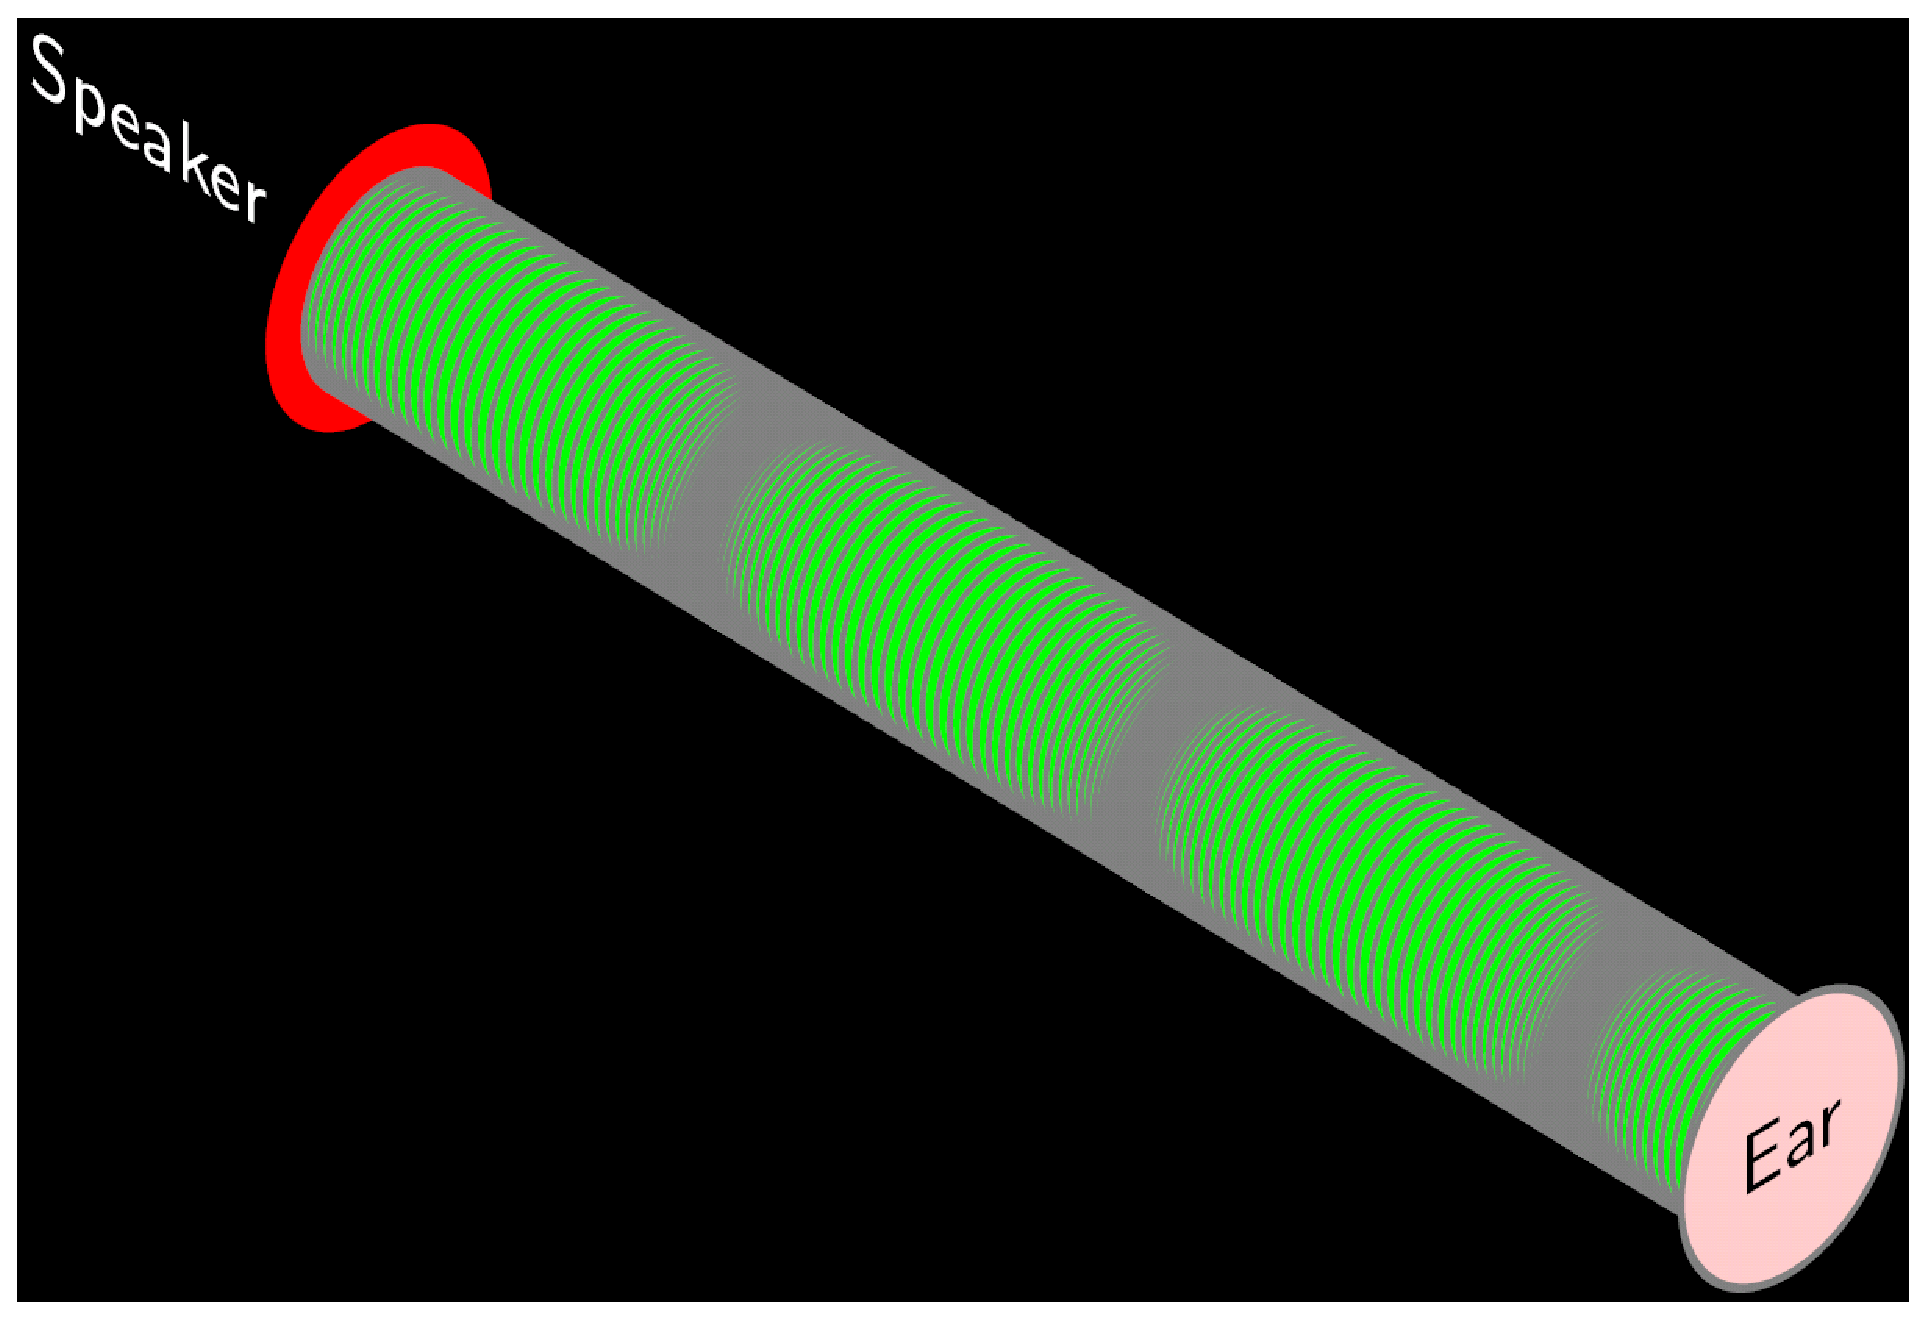
\includegraphics[width=2.2in]{pictures/soundbmp.eps}}
	\end{minipage}&
	\hspace{0.0in}
	\begin{minipage}[b]{1.2in}\textcolor{white}{%
	This image depicts air being compressed as sound waves in a tube from a speaker and then travelling through the tube towards the ear.\\	}
	\end{minipage}
	\end{tabular}
	\vspace{.2in}
}
